\chapter{Entscheidungsfindung} % (fold)
\label{cha:Entscheidungsfindung}

\section{Verwendete Methoden} % (fold)
\label{sec:Verwendete Methoden}

Verwendete Methoden
Um eine fundierte und stichhaltige Entscheidung treffen zu können und diese auch angemessen begründen zu können, haben wir uns für eine Nutzwertanalyse entschieden.

Eine Nutzwertanalyse ist eine Methode zur Entscheidungsfindung und wird häufig in komplexen Situationen verwendet, wenn beispielsweise viele verschiedene Aspekte und Meinungen betrachtet werden müssen. \footcite[Vgl.][S. 1 auch im Folgenden]{Kuhnapfel.2019} Sie beruht auf dem Prinzip der „Fragmentierung“, das bedeutet das Gesamtproblem wird in einzelne Teilprobleme aufgeteilt, die, wenn dies sinnvoll ist, noch einmal in ihre Teilprobleme aufgeteilt werden können. Dieses intuitive Modell wird häufig unterbewusst angewendet, wenn wir beispielsweise entscheiden wohin wir in den Urlaub möchten. Es können objektive Informationen, wie in diesem Beispiel Kosten oder Freizeitangebote, aber auch subjektive, wie Vorlieben für Essen oder Unterkunft betrachtet und miteinander abgewogen werden. \footcite[Vgl.][S. 43]{Dittmer.1995}

Durch das Erstellen einer Nutzwertanalyse wird dieser unterbewusste Prozess in den Vordergrund gebracht und der Fokus auf die Transparenz der Ergebnisse gelegt. Des Weiteren bewirkt die Fragmentierung eine Entemotionalisierung des Problems. Die Teilprobleme lenken von der emotionalen Bindung oder von einer spontanen Präferenz der Gesamtlösung ab und können leichter rational betrachtet und diskutiert werden. Dies ist vor allem der Fall, wenn der Anteil der Teillösung an der Gesamtlösung nicht klar ist. \footcite[Vgl.][S. 2]{Kuhnapfel.2019} Besonders der tendenziellen Präferenz sich für die Konstanz und gegen Veränderung zu entscheiden, wird hier entgegengewirkt.
Für eine zielführende Durchführung einer Nutzwertanalyse ist eine klar festgelegte Struktur notwendig, an der sich orientiert werden kann. Der erste und wichtigste Schritt ist die Ableitung des Zielsystems. \footcite[Vgl.][S. 44 f. auch im Folgenden]{Dittmer.1995} Ein Zielsystem setzt sich aus den bestimmten Kriterien zusammen und sollte eindeutige und objektive Beschreibungen der Wirkungen und Konsequenzen von Alternativen erlauben und alle relevanten Wertevorstellungen der Entscheidungsträger umfassen. Bei der Findung helfen Prozessfragen, wie beispielsweise „Welche Wirkungen werden beabsichtigt?“, „Worauf wirken die Alternativen?“, oder „Welche Wirkungen sollen vermieden werden?“.

Im Anschluss werden Ausschluss- und Auswahlkriterien definiert. Hier beginnt man mit Ausschlusskriterien, diese werden nicht in die Nutzwertanalyse mit einfließen, sondern schließen die Alternative kategorisch aus (auch K.O. Kriterien genannt). Auswahlkriterien können grundsätzlich in Leistungs-, Kosten-, und Terminkriterien eingeteilt werden, wobei in dieser Arbeit noch fachspezifische Kriterien betrachtet werden. \footnotemark
\footnotetext{Vgl. \cite{Wikipedia.2022} und \cite{FfEMunchen.2022}}
Eine Menge von 10-20 Kriterien wird als sinnvoll betrachtet, vor allem um zu verhindern, dass später besprochene Kriterien oberflächlicher behandelt und diskutiert werden als zu Beginn besprochene. \footcite[Vgl.][S. 8]{Kuhnapfel.2019}

Folgende Anforderungen werden an Kriterien in einer Nutzwertanalyse gestellt: \footnotemark
\footnotetext{Vgl. \cite{Kuhnapfel.2019} und \cite{Wikipedia.2022} auch im Folgenden}

\begin{description}
	\item \emph{Vollständigkeit:} Die Kriterien müssen das Problem vollständig umfassen, es darf also kein relevanter Aspekt für das Problem ausgelassen werden.
	\item \emph{Bewertbarkeit:} Kriterien sollten insofern bewertbar sein, als dass sie entweder qualitativ oder quantitativ erfassbar oder messbar sind, oder alle Teilnehmenden über das nötige Hintergrundwissen verfügen müssen, um eine informierte Bewertung abgeben zu können. Alternativ kann mit Enthaltungen gearbeitet werden, wenn beispielsweise ein sehr technischer und ein wirtschaftlicher Teil von zwei verschiedenen Abteilungen beurteilt wird.
	\item \emph{Relevanz:} Die Kriterien sollten für das in Frage stehende Problem relevant sein. Hier kann allerdings häufig keine eindeutige Aussage getroffen werden, da Teilnehmende hier eventuell andere Ansichten haben und oft keine objektive Antwort vorliegt.
	\item \emph{Reproduzierbarkeit:} Die verwendeten Kriterien sollten in ihrer Bewertung reproduzierbar sein. Das ist beispielsweise nicht der Fall, wenn die Verlässlichkeit einer Bank betrachtet wird und diese aktuell durch einen Sturm so verwüstet wurde, dass sie vorerst nicht handlungsfähig ist. Solange der Grund für die Unbeständigkeit nicht am Zielsystem selbst liegt ist das Kriterium unbrauchbar.
\end{description}

Im nächsten Schritt wird jedem Kriterium eine Gewichtung zu geordnet. Auch hier finden verschiedene Methoden Anwendung. Die einfachste aber auch ungenaueste Methode ist das „Ranking“, oder „Direct Ranking“. Hierbei wird jedem Kriterium ein Rang gegeben. Der Bereich der Aufstellung spielt hier keine große Rolle, ist im Beispiel (Abb. \ref{abb:DirectRanking}) aber mit 0-10 definiert.

\begin{figure}[htb]
	\centering
	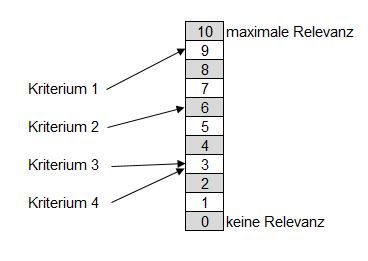
\includegraphics[width=5cm]{graphics/Direct_Ranking_Methode.JPG}
	\caption[Grafisches Beispiel Direct Ranking]{Grafisches Beispiel Direct Ranking. \footnotemark}
	\label{abb:DirectRanking}
\end{figure}
\footnotetext{Entnommen aus \cite{Wikipedia.2022}}

% section Verwendete Methoden (end)

% chapter (end)
